\documentclass[tikz,border=8pt]{standalone}
\usepackage{amsmath,amssymb}
\usetikzlibrary{calc,arrows.meta,patterns.meta}
% FLAT-GEOMETRY-V1 — publication authority
\definecolor{Ink}{HTML}{1E2933}
\definecolor{Muted}{HTML}{59636E}
\definecolor{Line}{HTML}{E0E5EA}
\definecolor{Violet}{HTML}{6D28D9}
\definecolor{Green}{HTML}{16823A}
\definecolor{GreenSoft}{HTML}{EAF5EE}
\definecolor{Red}{HTML}{CF222E}
\definecolor{Gold}{HTML}{8B5E00}

\newcommand{\regularpolygon}[4]{%
  \draw[#4,line width=0.8pt]
  \foreach \k in {0,...,#1} {
    \ifnum\k=0
      ($(#2)+({#3*cos(90+360*\k/#1)},{#3*sin(90+360*\k/#1)})$)
    \else
      -- ($(#2)+({#3*cos(90+360*\k/#1)},{#3*sin(90+360*\k/#1)})$)
    \fi
  };
}

\begin{document}
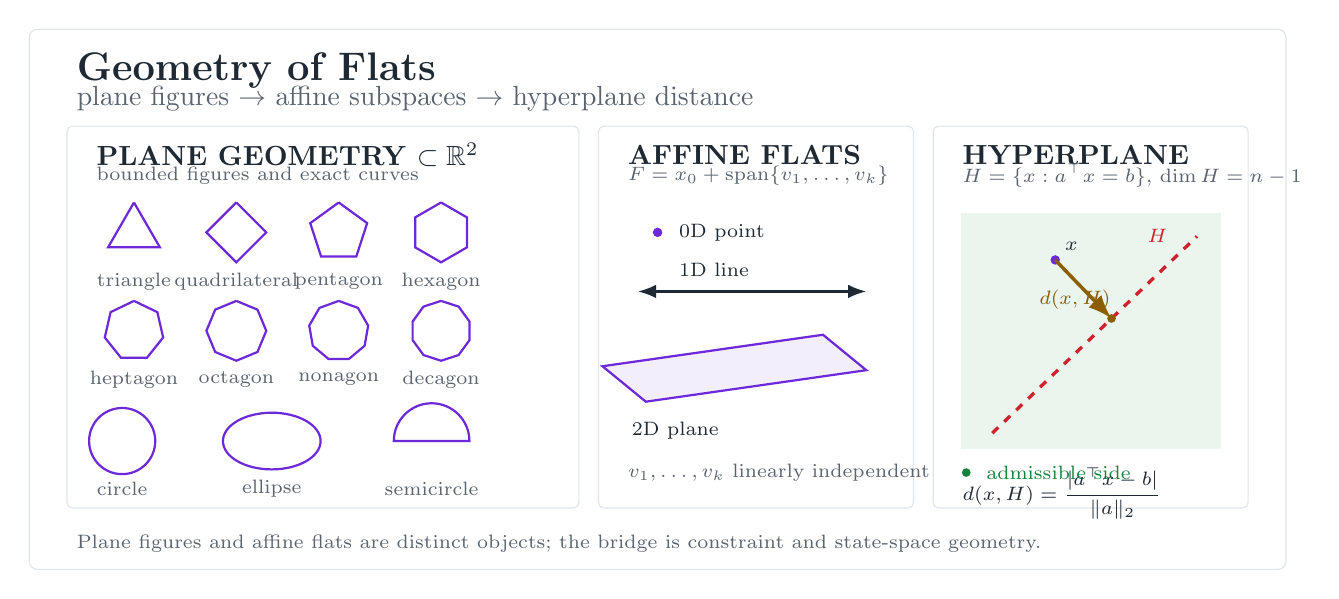
\begin{tikzpicture}[x=1cm,y=1cm,>=Latex,every node/.style={text=Ink}]
  \fill[white] (0,0) rectangle (16,6.9);
  \draw[Line,rounded corners=3pt] (0.02,0.02) rectangle (15.98,6.88);

  \node[anchor=west,font=\bfseries\Large] at (0.5,6.35) {Geometry of Flats};
  \node[anchor=west,text=Muted] at (0.5,6.0) {plane figures $\rightarrow$ affine subspaces $\rightarrow$ hyperplane distance};

  \draw[Line,rounded corners=2pt] (0.5,0.8) rectangle (7.0,5.65);
  \node[anchor=west,font=\bfseries] at (0.75,5.28) {PLANE GEOMETRY $\subset \mathbb R^2$};
  \node[anchor=west,text=Muted,font=\scriptsize] at (0.75,5.02) {bounded figures and exact curves};

  \foreach \n/\x/\y/\name in {
    3/1.35/4.3/triangle,
    4/2.65/4.3/quadrilateral,
    5/3.95/4.3/pentagon,
    6/5.25/4.3/hexagon,
    7/1.35/3.05/heptagon,
    8/2.65/3.05/octagon,
    9/3.95/3.05/nonagon,
    10/5.25/3.05/decagon}{
      \regularpolygon{\n}{\x,\y}{0.38}{Violet}
      \node[font=\scriptsize,text=Muted] at (\x,\y-0.62) {\name};
  }

  \draw[Violet,line width=0.8pt] (1.2,1.65) circle (0.42);
  \node[font=\scriptsize,text=Muted] at (1.2,1.05) {circle};
  \draw[Violet,line width=0.8pt] (3.1,1.65) ellipse (0.62 and 0.36);
  \node[font=\scriptsize,text=Muted] at (3.1,1.05) {ellipse};
  \draw[Violet,line width=0.8pt] (4.65,1.65) arc[start angle=180,end angle=0,radius=0.48] -- cycle;
  \node[font=\scriptsize,text=Muted] at (5.13,1.05) {semicircle};

  \draw[Line,rounded corners=2pt] (7.25,0.8) rectangle (11.25,5.65);
  \node[anchor=west,font=\bfseries] at (7.5,5.28) {AFFINE FLATS};
  \node[anchor=west,text=Muted,font=\scriptsize] at (7.5,5.02) {$F=x_0+\operatorname{span}\{v_1,\dots,v_k\}$};

  \fill[Violet] (8.0,4.3) circle (0.06);
  \node[anchor=west,font=\scriptsize] at (8.15,4.3) {$0$D point};

  \draw[Ink,line width=0.8pt,<->] (7.75,3.55) -- (10.65,3.55);
  \node[anchor=west,font=\scriptsize] at (8.15,3.82) {$1$D line};

  \fill[Violet!8] (7.85,2.15) -- (10.65,2.55) -- (10.1,3.0) -- (7.3,2.6) -- cycle;
  \draw[Violet,line width=0.8pt] (7.85,2.15) -- (10.65,2.55) -- (10.1,3.0) -- (7.3,2.6) -- cycle;
  \node[anchor=west,font=\scriptsize] at (7.55,1.78) {$2$D plane};

  \node[anchor=west,font=\scriptsize,text=Muted] at (7.5,1.25) {$v_1,\ldots,v_k$ linearly independent};

  \draw[Line,rounded corners=2pt] (11.5,0.8) rectangle (15.5,5.65);
  \node[anchor=west,font=\bfseries] at (11.75,5.28) {HYPERPLANE};
  \node[anchor=west,text=Muted,font=\scriptsize] at (11.75,5.02) {$H=\{x:a^\top x=b\}$, $\dim H=n-1$};

  \fill[GreenSoft] (11.85,1.55) rectangle (15.15,4.55);
  \draw[Red,dashed,line width=1.2pt] (12.25,1.75) -- (14.85,4.25);
  \node[text=Red,font=\scriptsize,anchor=west] at (14.1,4.25) {$H$};
  \fill[Violet] (13.05,3.95) circle (0.06) node[above right,font=\scriptsize] {$x$};
  \draw[Gold,->,line width=1.25pt] (13.05,3.95) -- (13.7648,3.2066);
  \fill[Gold] (13.7648,3.2066) circle (0.055);
  \node[text=Gold,font=\scriptsize] at (13.30,3.45) {$d(x,H)$};
  \fill[Green] (11.92,1.25) circle (0.055);
  \node[text=Green,font=\scriptsize,anchor=west] at (12.05,1.25) {admissible side};
  \node[anchor=west,font=\scriptsize] at (11.75,0.98)
    {$d(x,H)=\dfrac{|a^\top x-b|}{\|a\|_2}$};

  \node[anchor=west,text=Muted,font=\scriptsize] at (0.5,0.35)
    {Plane figures and affine flats are distinct objects; the bridge is constraint and state-space geometry.};
\end{tikzpicture}
\end{document}
